\documentclass[SE,authoryear,toc]{lsstdoc}
% \documentclass[SE,lsstdraft,authoryear,toc]{lsstdoc}

% lsstdoc documentation: https://lsst-texmf.lsst.io/lsstdoc.html
\input{meta}

% Package imports go here.

% Local commands go here.

%If you want glossaries
%\input{aglossary.tex}
%\makeglossaries

\title{Rubin Construction Documentation Inventory}

% Optional subtitle
% \setDocSubtitle{A subtitle}

\author{%
Chuck Claver (chair)
David Cabrera (co-Chair)
Rob McKercher (co-chair)
John Andrew
Diane Hascall
Patrick Ingraham
Tony Johnson
Kristen Metzger
Austin Roberts
Jonathan Sick
}

\setDocRef{SITCOMTN-012}
\setDocUpstreamLocation{\url{https://github.com/lsst-sitcom/sitcomtn-012}}

\date{\vcsDate}

% Optional: name of the document's curator
% \setDocCurator{The Curator of this Document}

\setDocAbstract{%
This tech note brings together the sources of critical documentation that has been developed across the Rubin Observatory Construction Project.  This inventory is meant as a guide to the Rubin Operations team for how and what documentation is transferred  as a deliverable from the construction Project
}

% Change history defined here.
% Order: oldest first.
% Fields: VERSION, DATE, DESCRIPTION, OWNER NAME.
% See LPM-51 for version number policy.
\setDocChangeRecord{%
  \addtohist{1}{2021-06-01}{Initial draft from Confluence pages.}{Chuck Claver}
}


\begin{document}

% Create the title page.
\maketitle
% Frequently for a technote we do not want a title page  uncomment this to remove the title page and changelog.
% use \mkshorttitle to remove the extra pages

% ADD CONTENT HERE
% You can also use the \input command to include several content files.

\section {Introduction}

As part of the second objective of \url{LSE-489.lsst.io}, this document represents the work of the Rubin Observatory Documentation Working Group in their survey of sources for construction and operations critical information and documents.  These sources include:

\begin{itemize}
	\item DocuShare;
	\item TechNotes from \url{lsst.io};
	\item Confluence Pages;
	\item Engineering Models; 
	\item GitHub Repositories;
	\item System-wide Databases;
	\item Verification Reports;
	\item Education and Public Outreach; 
	\item Information Technology; and
	\item Individual Storage; Slack Chat and Personal Repository Spaces.
\end{itemize}
	
There are additional document categories under development and continuous content updates to documents by Construction, Pre-operations and Operations Teams at the time of releasing \url{SITCOMTN-012.lsst.io}. This document may be revised to include updates to sources and documents as they are developed and matured; but this is not required. These include procedures for standard operations, regular maintenance, servicing and repair.

\newpage
\section{DocuShare}

Xerox\textregistered\ DocuShare\textregistered\ content management system \citep{DocuShare-cite} is the Construction Project's official document repository. It was selected during the design and development phase to meet the NSF requirement for a document management system. During Construction, the NSF requires retention of, at minimum, record of any decision affecting the cost, schedule or performance baseline. The NSF Major Facilities Guide specifies retention of a contingency log, change requests and approvals, and system integration, commissioning, testing and acceptance plans and results. During Operations, the NSF requires retention of documents related to facility performance in terms of maintenance, operating time, scheduled and unscheduled down time, and use for research and education. In addition to NSF requirements, the Project Office expects DocuShare to be the repository for official versions of management policies, plans and procedures, design documents, safety documentation, hazard analyses, released requirements and interface control documents generated from the SysML model, and project standards, guidelines and templates. The previous list is not intended to be exhaustive.

Three of DocuShare's advantages are handles, version control and co-location. Each object has a unique identifier called a handle, which follows the object regardless of versioning or location(s) in the directory structure (called collections). Each handle has a version history that lists all previously uploaded files for the object in question. One of those versions is designated as the preferred version, which represents the document's official, approved version and is served by the database when clicking the object's title or from a properly formatted URL shared or hosted outside of DocuShare. The object's handle does not change when/if a new version of the document is created. Lastly, objects can appear simultaneously in as many collections as are necessary and/or relevant to the document. This is facilitated by an object's "locations" property; locations are added as appropriate, and the handle automatically appears in the newly added locations. The combination of handles, versioning and co-location creates a system where each document is represented by a single record, avoiding duplication and/or version confusion.

Currently, DocuShare contains more than 30,000 documents in more than 10,000 collections. A high-level survey of DocuShare shows retention of 1) requirements, designs, interfaces, policies and plans under change control - whether controlled at the project- or subsystem-level; 2) change control action records; 3) status reports to NSF, AURA and other stakeholders; 4) safety standards, accidents reports and investigations documentation; 5) hazard mitigation verification artifacts; 6) risk reports; and 7) project-level review agendas, presentations and reference documents. Creation, retention and version control of those documentation classes generally have been well managed; however, the bulk of DocuShare documents likely represents objects created ad hoc by general project staff for specific purposes. In addition, there are thousands of pieces of work product that may have archival significance but likely will not be useful for Operations.

As part of the Rubin Observatory Document Working Group effort, a study was conducted to evaluate the future use of DocuShare into Operations.  The DocuShare Options Trade Study \citedsp{Document-36788} is found at \url{ls.st/Document-36788}, and includes an examination of the following use cases:

\begin{itemize}
	\item Using the Existing Rubin Observatory Project DocuShare instance with modifications;
	\item Extending Rubin Observatory Project DocuShare with Archiver Server Enabled; and
	\item Adopting the NOIR Laboratory DocuShare instance.
\end{itemize}

\newpage
\section{TechNotes: https://www.lsst.io}

LSST the Docs (LTD), also known by its URL "lsst.io", is a documentation hosting platform built and operated by the SQuaRE (Data Management) team. LTD hosts what are called static websites, meaning any website built from HTML, CSS and JavaScript that doesn't need an active server to render content (as opposed to say Confluence, DocuShare, or Drupal websites). Static websites are a natural fit for documentation projects that originate from a GitHub repository, such as software documentation or LaTeX documents. Teams use the same processes to collaborate on documentation as they are with code, and the documentation is tested and built using the same process as the software is tested and built. LTD is unique in that is it built around versioned documentation. The root URL for a documentation project hosts the "default" version (which has a configurable meaning for each project). The user can also browse other versions of the documentation through the "/v/" dashboard pages (for example \url{https://www.lsst.io/v/}). Versions might correspond to software release versions or to temporary collaborative drafts corresponding to GitHub Pull Requests.

The homepage for the documentation platform, \url{https://www.lsst.io}, serves as a portal for documentation. \citep{lsst.io-cite} Users can search across metadata and full text (this feature is powered by the commercial service Algolia \citep{Algolia-cite} in conjunction with a scraper bot built by SQuaRE) or browse through curated collections. As \url{https://www.lsst.io} is a site designed and built by the SQuaRE team, there is considerable opportunity to refine the design of the portal to meet the specific needs of Rubin Observatory. It is also possible for the portal to list and provide search functionality for documentation hosted on other platforms (potential examples include Confluence, DocuShare, and the acronyms/terminology database).

From a technical perspective, LTD hosts two types of documentation projects: guides and documents. Guides are multi-page websites. The guideline in the DM subsystem is that every software project or service has a guide hosted on lsst.io. An example of a DM guide for a software project is \url{https://pipelines.lsst.io} and a guide for a service is \url{https://nb.lsst.io}. T\&S is also hosting software guides: see \url{https://obs-controls.lsst.io} as an example. Besides documentation tied to specific software projects or services, guides can also collect procedures for teams, see the DM Developer Guide (\url{https://developer.lsst.io}) or the Observatory Operations Documentation (\url{https://obs-ops.lsst.io}). Though not required, guides are generally authored using an open-source tool called Sphinx \citep{Sphinx-cite} using a theme that is maintained by the SQuaRE team. The second type of documentation, documents, are "single-page" artifacts that are analogous to documents that might be found in DocuShare. Indeed, DM has taken to developing most of its LDM change-controlled documents on its lsst.io site to take advantage of the sophisticated collaboration features that GitHub offers (for an example, see \url{https://ldm-151.lsst.io}). \citep{GitHub-cite} Change-controlled documents are submitted to DocuShare for archival once approved using a release process mediated through GitHub, Jira, and the relevant control board. LTD is currently hosting documents from the DMTR, LDM, LPM, LSE, and SCTR document series (note that this includes test and verification reports). Besides change-controlled documents, Rubin Observatory project members can also author informal documents called technical notes. Technical notes were introduced as a medium that blended the organization of DocuShare documents (documents have unique handles) with the ease of Confluence (staff can author and publish technical notes independently without assistance or overt oversight). 

Technical notes series are associated with different subsystems and include DMTN, ITTN, PSTN, RTN, SITCOMTN, SMTN, SQR, and TSTN. Counts of the number of available documents of each type are listed in the table below, as of June 2021:

\begin{longtable}{p{0.2\textwidth}p{0.2\textwidth}}\hline
\textbf{Content Type} & \textbf{Document Count}  \\\hline
Guides		& 59 		\\\hline
DMTN 		& 172	\\\hline
DMTR		& 22 		\\\hline
ITTN		& 34 		\\\hline
LDM			& 38 		\\\hline
LPM 		& 2 		\\\hline
PSTN  		& 51  	\\\hline
RTN   		& 12 		\\\hline
SCTR 		& 8 		\\\hline
SITCOMTN	& 12 		\\\hline
SMTN 		& 14		\\\hline
SQR 		& 49 		\\\hline
TSTN 		& 25          \\\hline          
\end{longtable}

\subsection{Terminology}

{\bf lsst.io:}  The documentation hosting domain for Rubin Observatory, which is powered by LSST the Docs. All subdomains of lsst.io are independent documentation projects (for example, developer.lsst.io for the DM Developer Guide or sqr-006.lsst.io for the SQR-006 technote).

{\bf \url{www.lsst.io}:}  The documentation portal. This is a regular documentation project hosted on lsst.io, but it uses the "www" subdomain to serve as a documentation homepage. \url{www.lsst.io} provides documentation search and faceted browsing capabilities. It is still in development and the current status is documented at \url{https://www.lsst.io/about/}. The site itself is built with React/Gatsby.js (\url{https://github.com/lsst-sqre/www_lsst_io}), the search database is SaaS \citep{SaaS-cite}), and the bot that indexes content into the search database is called Ook (\url{https://github.com/lsst-sqre/ook}).

{\bf LSST the DOCS (LTD):}  Commonly written as LTD, LSST the Docs is the technical system for hosting versioned static websites. lsst.io is one such deployment. The technical motivation and design of LTD are documented in SQR-006: The LSST the Docs Platform for Continuous Documentation Delivery (\url{https://sqr-006.lsst.io}, \citeds{SQR-006}). The key technical features of LTD are:

\begin{itemize}
	\item High reliability, scaling, and security: documentation is hosted in Amazon S3 and served through the Fastly content distribution network. We don't operate any servers that receive traffic from users;
	\item Versioned documentation; and
	\item Flexibility to host any type of static website.
\end{itemize}

{\bf Technical notes (technotes):}  These are documents that are not change controlled, but otherwise have features similar to "official" project documents. They were designed by the DM SQuaRE team as a replacement for Confluence in writing organized documents for sharing ideas within, and beyond, the project. See SQR-000: The LSST DM Technical Note Publishing Platform (https://sqr-000.lsst.io) for our motivation to create technical notes. \citedsp{SQR-000}

\newpage
\section{Confluence Pages}

Confluence is used by the by the construction Project for many purposes.  Confluence is primarily a collaborative tool where teams/groups can document and share and develop information.  The tool is organized in "work spaces" for which the Project currently has 34 defined spaces.  Many of these spaces are very specialized or have been set up for personal use.  In this section we limit ourselves to those spaces that are directly related to the deliverables from the integrated Rubin Construction Project spanning of two independent repositories -- one served out of Tucson for the MREFC effort and another served out of SLAC for the DOE MIE LSSTCam effort.

Most of the pages linked here requireRubin Construction Project credential for access.

\begin{small}

\subsection{Tucson based MREFC Spaces}

\begin{itemize}
	\item \href{https://confluence.lsstcorp.org/display/PC/Project+Management+Controls+System+Home}{Project Management Controls}
	\item \href{https://confluence.lsstcorp.org/display/PS/Project+Science+Home}{Project Science}
	\item \href{https://confluence.lsstcorp.org/display/ROA/Rubin+Obs.+Admins}{Rubin Admin.}
	\item \href{https://confluence.lsstcorp.org/pages/viewpage.action?pageId=48399826}{System, Integration, Test \& Commissioning}
	\begin{itemize}
		\item \href{https://confluence.lsstcorp.org/display/LSSTCOM/SIT-Com+Management?src=contextnavpagetreemode}{SIT--Com Management}
		\item \href{https://confluence.lsstcorp.org/display/LSSTCOM/SIT-Com+Planning?src=contextnavpagetreemode}{SIT--Com Planning}
		\item \href{https://confluence.lsstcorp.org/display/LSSTCOM/SIT-Com+Activities?src=contextnavpagetreemode}{SIT--Com Activities}
		\item \href{https://confluence.lsstcorp.org/display/LSSTCOM/SIT-Com+Science+Verification?src=contextnavpagetreemode}{SIT--Com Science Verification}
		\item\href{https://confluence.lsstcorp.org/display/LSSTCOM/SIT-Com+Requirements+for+Operations?src=contextnavpagetreemode}{SIT--Com Requirements for Operations}
		\item \href{https://confluence.lsstcorp.org/display/LSSTCOM/DOE+Notes?src=contextnavpagetreemode}{SIT--Com DOE Notes}
	\end{itemize}
	\item \href{https://confluence.lsstcorp.org/display/SYSENG/Systems+Engineering+Home}{Systems Engineering}
	\begin{itemize}
		\item \href{https://confluence.lsstcorp.org/pages/viewpage.action?pageId=97681640}{Failure Report, Analysis and Corrective Action System}
		\item \href{https://confluence.lsstcorp.org/pages/viewpage.action?pageId=100173626}{Verification \& Validation Documentation}
		\item \href{https://confluence.lsstcorp.org/display/SYSENG/Hazard+Mitigation+Verification+Documentation}{Hazard Verification Documentation}
		\item \href{https://confluence.lsstcorp.org/display/RM/Risk+Management+on+JIRA}{Risk Management}
		\item \href{https://confluence.lsstcorp.org/pages/viewpage.action?pageId=3113550}{Telescope \& Site Change Control}
		\item MagicDraw importing, setup, usage instructions
	\end{itemize}
	\item \href{https://confluence.lsstcorp.org/display/DM/Data+Management+Home}{Data Management}
	\begin{itemize}
		\item \href{https://confluence.lsstcorp.org/display/LSP/Science+Platform+Operations+Home}{Rubin Science Platform}
	\end{itemize}
	\item \href{https://https//confluence.lsstcorp.org/pages/viewpage.action?pageId=1507765}{Telescope \& Site}
	\item \href{https://confluence.lsstcorp.org/pages/viewpage.action?pageId=25690606}{Education \& Public Outreach}
	\item \href{https://confluence.lsstcorp.org/display/LKB/Rubin+Lessons+Learned}{Rubin Observatory Knowledge Base}
\end{itemize}

\subsection{SLAC Based LSSTCam Spaces}
These pages require SLAC LSSTCam credentials.

\begin{itemize}
	\item \href{https://confluence.slac.stanford.edu/display/LSSTCAM}{Primary LSSTCam Space}
	\item \href{https://confluence.slac.stanford.edu/pages/viewpage.action?pageId=130884078}{LSSTCam Safety \& Hazards}
	\begin{itemize}
		\item LSSTCam Subsystem Pages
		\begin{itemize}
			\item \href{https://confluence.slac.stanford.edu/display/LSSTCAM/3.01+Project+Management}{LSSTCam Project Management (3.01)}
			\item \href{https://confluence.slac.stanford.edu/display/LSSTCAM/3.02+Camera+Systems+Integration}{LSSTCam Systems Integration (3.02)}
			\item \href{https://confluence.slac.stanford.edu/display/LSSTCAM/3.03+Sensors}{LSSTCam Sensors (3.03)}
			\item \href{https://confluence.slac.stanford.edu/display/LSSTCAM/3.04.01+Camera+Science+Raft}{LSSTCam Science Rafts (3.04.01)}
			\item \href{https://confluence.slac.stanford.edu/display/LSSTCAM/3.04.02+Corner+Rafts}{LSSTCam Corner Rafts (3.04.02)}
			\item \href{https://confluence.slac.stanford.edu/display/LSSTCAM/3.05+Optics}{LSSTCam Optics (3.05)}
			\item \href{https://confluence.slac.stanford.edu/display/LSSTCAM/3.06.01-.02+Camera+Body+and+Shutter}{LSSTCam Body \& Shutter (3.06.01)}
			\item \href{https://confluence.slac.stanford.edu/display/LSSTCAM/3.06.02+Shutter}{LSSTCam Shutter (3.06.02)}
			\item \href{https://confluence.slac.stanford.edu/display/LSSTCAM/3.06.03+Exchange+System}{LSSTCam Exchange System (3.06.03)}
			\item \href{https://confluence.slac.stanford.edu/display/LSSTCAM/3.06.04+Cryostat}{LSSTCam Cryostat (3.06.04)}
			\item \href{https://confluence.slac.stanford.edu/display/LSSTCAM/3.07.01+Camera+Control+System}{LSSTCam Control System (3.07.01)}
			\item \href{https://confluence.slac.stanford.edu/display/LSSTCAM/3.07.02+Data+Acquisition}{LSSTCam Data Acquisition System (3.07.02)}
			\item \href{https://confluence.slac.stanford.edu/display/LSSTCAM/3.07.03+Auxiliary+Electronics}{LSSTCam Auxiliary Electronics (3.07.03)}
			\item \href{https://confluence.slac.stanford.edu/display/LSSTCAM/3.08+Integration+and+Test}{LSSTCam Integration and Test (3.08)}
		\end{itemize}
		\item LSSTCam Group Pages
		\begin{itemize}
			\item \href{https://confluence.slac.stanford.edu/display/LSSTCAM/Camera+Database+and+Data+Management}{LSSTCam Databases \& Management}
			\item \href{https://confluence.slac.stanford.edu/pages/viewpage.action?pageId=132230553}{Sensor Characterization \& Testing}
			\item \href{https://confluence.slac.stanford.edu/display/LSSTCAM/Commissioning+Camera}{ComCam (DOE)}
			\item \href{https://confluence.slac.stanford.edu/display/LSSTCAM/Auxiliary+Telescope}{Auxiliary Telescope (DOE)}
			\item \href{https://confluence.slac.stanford.edu/display/LSSTCAM/General+Computing}{LSSTCam General Computing}
			\item \href{https://confluence.slac.stanford.edu/display/LSSTCAM/Refrigeration+and+the+TMA}{LSSTCam Refrigeration \& TMA}
			\item \href{https://confluence.slac.stanford.edu/display/LSSTCAM/Commissioning+and+Early+Operations}{LSSTCam Commissioning \& Early Operations}
		\end{itemize}
		\item \href{https://confluence.slac.stanford.edu/display/LSSTCAM/Camera+Policies+and+Procedures}{LSSTCam Policies \& Procedures}
		\item Other LSSTCam pages
		\begin{itemize}
			\item \href{https://confluence.slac.stanford.edu/display/LSSTCAM/Site+Indexes+and+Libraries}{LSSTCam Libraries}
			\item \href{https://confluence.slac.stanford.edu/display/LSSTCAM/LSSTCAM+Site+Indexes}{LSSTCam Indexes}
			\item \href{https://confluence.slac.stanford.edu/display/LSSTCAM/Camera+Working+Documents+Lists}{LSSTCam Document Lists}
			\item \href{https://confluence.slac.stanford.edu/display/LSSTCAM/Camera+Document+Status}{LSSTCam Document Status}
			\item \href{https://confluence.slac.stanford.edu/pages/viewpage.action?pageId=165088106}{LSSTCam Images \& Photos}
			\item \href{https://confluence.slac.stanford.edu/display/LSSTCAM/Technical+Notes}{LSSTCam Technical Notes}
			\item \href{https://confluence.slac.stanford.edu/pages/viewpage.action?pageId=145032457}{LSSTCam Past Events \& Review (2013)}
			\item \href{https://confluence.slac.stanford.edu/pages/viewpage.action?pageId=138800070}{LSSTCam Upcoming Events}
			\item \href{https://confluence.slac.stanford.edu/pages/viewpage.action?pageId=126522700}{Workshop \& Meetings}
		\end{itemize}
	\end{itemize}
	\item \href{https://confluence.slac.stanford.edu/display/LSSTCAMREV}{LSSTCam Review Space}
	\item \href{https://confluence.slac.stanford.edu/display/LSSTCAML4/LSST+Camera+CCD+e2v+Vendor+Working+Group+Home}{E2V Sensor Development Material (restricted, NDA required)}
	\item \href{https://confluence.slac.stanford.edu/display/LSSTCAMI/LSST+Camera+Vendor+1+Working+Group+Home}{ITL Sensor Development Material (restricted, NDA required)}
\end{itemize}

\end{small}
\newpage
\section{Engineering Models}

Solidworks Product Data Management (PDM) Professional \citep{PDM-cite} is the Telescope and Site group's official CAD model repository. It was selected during the design and development phase to meet the NSF requirement for configuration management of the baseline mechanical engineering design. The software uses a check-out / check-in system to allow configuration management of the design. Each check-in produces a new version of the part or assembly. Earlier versions can be accessed if needed to compare designs or revert to an earlier design. A workflow feature allows the designs to go through a review process until the design is approved and locked from further changes. A revision process is also included in the workflow to allow for changes to the designs if needed after final approval. The software allows for vault replication at multiple sites and the project currently has a server operating in Tucson and Chile to support CAD users at multiple sites.

The PDM system currently stores all the Telescope and Site group's CAD models of the original mechanical baseline design. The CAD models are linked to a series of ICD documents (drawings) describing the mechanical interfaces for the different optical and mechanical subsystems of the observatory. In addition to the baseline design models, the PDM system contains CAD models of the as-designed and as-built CAD models from the subsystem vendors. Complete designs and documentation of subsystems completed by the Telescope and Site group are also included. In addition to CAD models a series of design and drafting standards is also stored in the PDM system.

The PDM system currently contains all design work created by the Telescope and Site group from early design and development through construction. No information has been deleted or archived at this time. The PDM system will be needed by the Operations team as the observatory goes through its design lifecycle of revisions and upgrades. A reorganization of the PDM vault to archive obsolete information is envisioned at the end of the construction phase of the project.

Rubin Observatory PDM Vault contents includes:

\begin{itemize}
	\item {\bf Original Project Baseline Design Documentation}
	\begin{itemize}
		\item ICD drawings for original requirements documents
		\item CAD models of T\&S subsystems baseline design
		\item Library of CAD models contains commercial off the shelf parts
		\item Template files
		\begin{itemize}
			\item Project drawing sheets, part files and assemblies template files
			\item Project dimension standard files for Solidworks
			\item Project Tables (BML, Revision, hole tables, etc.)
		\end{itemize}
	\end{itemize}

	\item {\bf Complete designs (models \& drawings) for subsystems completed by the T\&S group}
	\begin{itemize}
		\item M1M3 mirror cell assembly
		\item M2 cone baffle
		\item Miscellaneous handling fixtures
		\item ComCam Assembly
	\end{itemize}

	\item {\bf CAD models of T\&S subsystems from vendor contracts}
	\begin{itemize}
		\item Telescope Mount Assembly (FDR Model)
		\item M2 Cell Assembly
		\item M2 Hexapod Assembly
		\item Camera Hexapod \& Rotator Assembly
		\item Dome (FDR model)
		\item Coating Plant
		\item Auxiliary Telescope \& Instrumentation
		\item Summit Facility includes Auxiliary Telescope Facility
	\end{itemize}

	\item{\bf CAD model of SLAC Camera assembly} (last update July 2013)  Add description of the process for synchronizing the LSSTCam CAD model here

\end{itemize}

\newpage
\section{GitHub}

The Rubin Observatory uses GitHub for software and documentation collaboration. The Observatory uses a large number of GitHub repositories, primarily to ease access control. As such, each construction subsystem generally has its own GitHub organization, though in some cases subsystems have additional GitHub organizations for specific teams or projects. The main GitHub organization (github.com/lsst) contains all software components officially released by the Data Management Subsystem (i.e., the Science Pipelines), and as such it serves as the public face of the observatory for astronomers interested in Rubin/LSST software. Not all operations software is found in the "lsst" organization, though. For example, Science Platform software is contained in "lsst-sqre," Telescope \& Site software in "lsst-ts," EPO software in "lsst-epo," and camera software in several organizations.

GitHub organizations with operational software and documentation will likely transition smoothly to operations teams. Particular attention will need to be paid to maintaining organizations that no longer have an active team associated with them.

\begin{small}

\begin{longtable}{p{0.175\textwidth}p{0.175\textwidth}p{0.175\textwidth}p{0.4\textwidth}}\hline
\textbf{Organization} & \textbf{Subsystem(s)} & \textbf{Documents} & \textbf{Notes}\\\hline
\href{https://github.com/lsst}{lsst}		& DM, PM, SIT--Com	&	LPM, LSE, LDM, RTN	&	LSST Science Pipelines and change-controlled documents. See DMTN-104 (DM product tree) \\\hline
\href{https://github.com/lsst-camera-ccs}{lsst-camera-ccs}			& LSSTCam	& &	Camera Control System (semi-private). See also LSST CCS release management \\\hline
\href{https://github.com/lsst-camera-daq}{lsst-camera-daq}		& LSSTCam 	& &	Camera DAQ (private) \\\hline
\href{https://github.com/lsst-camera-dh}{lsst-camera-dh}			& LSSTCam  	& &	Camera Data Handling+eTraveler+misc scripts+sequencers \\\hline
\href{https://github.com/lsst-camera-electronics}{lsst-camera-electronics}	& LSSTCam	& &	Camera firmware \\\hline
\href{https://github.com/lsst-camera-visualization}{lsst-camera-visualization}	& LSSTCam	& &	Camera visualization (image display) \\\hline
\href{https://github.com/lsst-dm}{lsst-dm}				& DM		& 	DMTN, DMTR	& DM workspace for technical notes, non-pipeline packages, unofficial and "legacy" pipelines packages \\\hline
\href{https://github.com/lsst-dmsst}{lsst-dmsst|}				& DM		& & 	DM System Science Team \\\hline
\href{https://github.com/lsst-dm-tutorial}{lsst-dm-tutorial}			& DM		& &	DM tutorials (mostly for authenticating workshop attendees and notebooks) \\\hline
\href{https://github.com/lsst-epo}{lsst-epo}				& EPO		& &	Education and Public Outreach \\\hline
\href{https://github.com/lsst-it}{lsst-it}					& IT			&	ITTN		& IT-related projects \\\hline
\href{https://github.com/lsst-opsim}{lsst-opsim}				& SIT--Com	& &	LSST Operations Simulator \\\hline
\href{https://github.com/lsst-pst}{lsst-pst}				& PST		& PSTN	& Project Science Team \\\hline
\href{https://github.com/lsst-se}{lsst-se}				& SIT--Com	& &	Systems Engineering \\\hline
\href{https://github.com/lsst-sims}{lsst-sims}				& SIT--Com	& SMTN	& LSST Simulations Group \\\hline
\href{https://github.com/lsst-sitcom}{lsst-sitcom}			& SIT--Com	& SCTR, SITCOMTN	& System Integration, Test, and Commissioning \\\hline
\href{https://github.com/lsst-sqre}{lsst-sqre}				& DM		& SQR	& DM SQuaRE (Science Platform, SQuaRE, and documentation infrastructure) \\\hline
\href{https://github.com/lsst-ts}{lsst-ts}				& TS			& &	Telescope \& Site \\\hline
\href{https://github.com/lsst-tstn}{lsst-tstn}				& TS			& TSTN	& Telescope \& Site  technical notes \\\hline
\href{https://github.com/rubin-observatory}{rubin-observatory}		& PMO		& &	Ops and pre-ops management documentation \\\hline

\end{longtable}

\end{small}
% \newpage
\section{System Databases}

Needs an introductory paragraph here.

\subsection{MagicDraw}

MagicDraw \citep{MagicDraw-cite} is a tool used by the project to maintain a model of the Rubin Observatory system creating a relational database between system elements.  Developed through the Rubin Observatory's use of MagicDraw, user guides are collected on the following Project confluence page: \href{https://confluence.lsstcorp.org/display/SYSENG/MagicDraw+LSST+Users+Guide}{MagicDraw Users Guide}.

The system elements captured with the MagicDraw database include:

\begin{itemize}
	\item Hazard Analysis - imported from various vendor and internal spreadsheets and now source of truth. Synced to Jira for verification
	\item FMEA - imported from various vendor and internal spreadsheets and now source of truth (currently incomplete)
	\item Requirements - source of truth with exports to DocuShare
	\item Verification Elements - source of truth for requirements details, synced to/from Jira
	\item Verification Plans/Cycles/Cases - synced to/from Jira, not source of truth
	\item SAL Commands, Events, Telemetry - imported from CSC XML
	\item Operations Concepts - source of truth
	\item System level state machine - source of truth
	\item Interlocks - modeled from source material
	\item Structural decomposition - sync from SolidWorks in the future
\end{itemize}

\subsection{JIRA}

JIRA is used by the by the Construction Project for many purposes.  JIRA is primarily a issue tracking tool where teams/groups can document, organize, track and report on software or administrative tasks. \citep{JIRA-cite} The tool is organized in "work spaces" called projects, each of which tracks a list of enumerated tickets or issues. JIRA provides a wide variety of tools to manipulate or organize projects and tickets. Many of these projects are very specialized or have been set up for personal use.  Listed below are projects related to the deliverables from the integrated Rubin Construction Project spanning of two independent repositories - one served out of Tucson for the MREFC effort and another served out of SLAC for the DOE MIE LSSTCam effort.

Need introductory/summary paragraph here about Tucson-based JIRA Projects.

\begin{itemize}
	\item Verification Elements/Plans/Cycles/Cases/Results - source of truth
	\item Risks, Opportunities, Mitigations - source of truth
	\item FRACAS - Failures, corrective actions - source of truth
	\item Hazard mitigation verification
\end{itemize}

Need introductory/summary paragraph here about LSSTCam-based JIRA Projects.
The list below collects JIRA projects within the SLAC-based JIRA instance. These items require SLAC LSSTCam credentials.

\begin{itemize}
	\item \href{https://jira.slac.stanford.edu/browse/LCAI}{Camera Action Items}: Captures action items for all Camera Subsystems, from various sources (reviews, internal discussions, etc.). Utilization is described on this confluence page: \href{https://confluence.slac.stanford.edu/pages/viewpage.action?pageId=130884357}{Using JIRA and Confluence to track Action Items}.
	\item \href{https://jira.slac.stanford.edu/browse/LSSTTD}{Test Data Framework}:  Spans many purposes, includes (not exclusive) reporting \href{http://lsst-camera.slac.stanford.edu/DataPortal/}{Data Portal}, \href{http://srs.slac.stanford.edu/DataCatalog/?experiment=LSST-CAMERA}{Data Catalog}, CCS initiated analyses, limitations, improvements (web-app or otherwise), eTraveler or database impacts (typically data structure related or new implementations).
	\item Camera Control System Core
	\begin{itemize}
		\item \href{https://jira.slac.stanford.edu/browse/LSSTCCS}{CCS Core}:  Self-explanatory.
		\item \href{https://jira.slac.stanford.edu/browse/LSSTCCSDRIVER}{CCS Driver}:  Driver development for using specific software/equipment with CCS.
		\item \href{https://jira.slac.stanford.edu/browse/LSSTCCSSUB}{CCS Subsystem}:   Not sure the difference between this and CCS Core.
		\item \href{https://jira.slac.stanford.edu/browse/LSSTCCSPROJ}{CCS Project}:  Old project; as stated by \href{https://jira.slac.stanford.edu/browse/LSSTCCSPROJ-80}{LSSTCCSPROJ-80}, it is replaced by CCS Core; but unsure if all tickets were migrated (open or closed).
		\item \href{https://jira.slac.stanford.edu/browse/LSSTCCSDOC}{CCS Documentation}:  Old project, few tickets remain open.
	\end{itemize}
	\item CCS Camera Subsystem and Interfaces Related
		\begin{itemize}
		\item \href{https://jira.slac.stanford.edu/browse/LSSTCCSPOWER}{CCS Power Manager Subsystem}:  self-explanatory.
		\item \href{https://jira.slac.stanford.edu/browse/LSSTCCSRAFTS}{CCS Rafts}:  self-explanatory.
		\item \href{https://jira.slac.stanford.edu/browse/LSSTCCSREFRIG}{CCS Refrigerator}:  self-explanatory.
		\item \href{https://jira.slac.stanford.edu/browse/LSSTCCSSHUTTER}{CCS Shutter}:  self-explanatory.
		\item \href{https://jira.slac.stanford.edu/browse/LSSTCCSUT}{CCS Utility Trunk}:  self-explanatory.
		\item \href{https://jira.slac.stanford.edu/browse/LCOBM}{CCS OCS Bridge and MCM}:  self-explanatory.
		\item \href{https://jira.slac.stanford.edu/browse/LSSTCCSDAQ}{CCS DAQ}:  self-explanatory.
		\item \href{https://jira.slac.stanford.edu/browse/LSSTCCSFCS}{CCS FCS}:  self-explanatory (FCS - filter change system?).	
	\end{itemize}
	\item CCS and Specific Applications
	\begin{itemize}
		\item \href{https://jira.slac.stanford.edu/browse/LSSTCCSTS}{CCS Test Stands}:  use of and item-specific items for test stands at various sites.
		\item \href{https://jira.slac.stanford.edu/browse/LSSTIR}{CCS IR2 Infrastructure}:  self-explanatory (IR2 is the SLAC Cleanroom).
		\item \href{https://jira.slac.stanford.edu/browse/LSSTCCSCOM}{CCS ComCam}:  self-explanatory, but issues not exclusive to this JIRA project.
	\end{itemize}
	\item \href{https://jira.slac.stanford.edu/browse/LSSTDREB}{DREB Firmware}:  8 tickets (all resolved) for DREB.
	\item \href{https://jira.slac.stanford.edu/browse/ETCCB}{eTraveler CCB}:  Changes to instructions, local software changes (Job Harness/Install), and a few decisions about how eTraveler was organized/implemented (software and hardware). See the following confluence page for context on CCB use: \href{https://confluence.slac.stanford.edu/display/LSSTCAM/eTraveler+CCB}{eTraveler CCB}
\end{itemize}

\subsection{Drupal}

Need introductory/summary paragraph here, with reference to figure (may not be on same page).

\begin{itemize}
	\item Change Control What resides in Drupal that is not in DocuShare?
	\item Review materials
	\item Are the review material fully captured in Docushare?  Yes, for Project level reviews.
	\item Open question regarding lower level reviews.
	\item Historical WEB pages
\end{itemize}

\subsection{Euporie}

Need introductory/summary paragraph here, with reference to figure (may not be on same page).

\begin{figure}
\begin{center}
  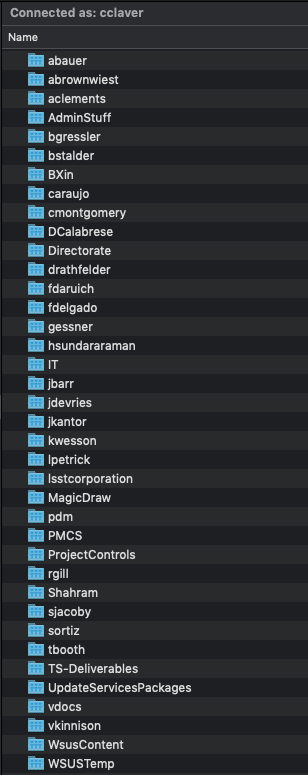
\includegraphics[scale=0.5]{Figures/EuporieDirectory.png}
\end{center}
\caption{\label{fig:EuporyDirectory} The current (June 2021) directory structure of the Euporie remote drive repository}
\end{figure}

\begin{figure}
\begin{center}
  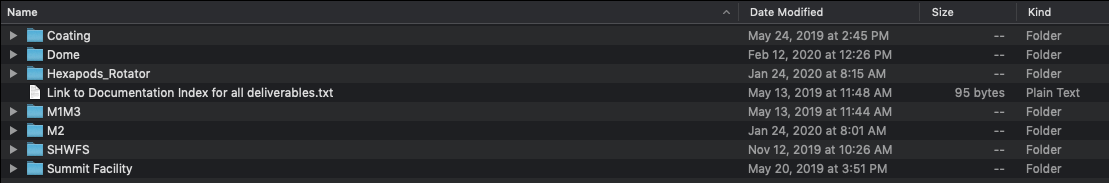
\includegraphics[scale=0.33]{Figures/EuporieTS.png}
\end{center}
\caption{\label{fig:EuporyTS} The Telescope \& Site folders on the Euporie repository used to collect documents from vendors}
\end{figure}

\subsection{T\&S Commandable SAL Component XML Files}

The T\&S XML package defines the data objects for all Commandable SAL Components (CSC). These data objects are defined in XML. SAL consumes the XML to produce language specific libraries that enable communication over the DDS network.  These XML files are critical for defining the configuration and interaction of the systems within the Summit Facility observing environment.

A link to the T\&S TechNote covering the XML files is here: \url{https://ts-xml.lsst.io}

\subsection{LSSTCam}
	\subsubsection{eTraveler}
	eTraveler is a web-based tool used across multiple sites during the testing and construction of the Camera and its subcomponents. It was used to provide procedures, begin testing and data collection locally, upload information and data to servers (primarily to the \href{http://lsst-camera.slac.stanford.edu/DataPortal/}{Data Portal} and \href{http://srs.slac.stanford.edu/DataCatalog/?experiment=LSST-CAMERA}{Data Catalog}), track component/assembly information, and track the acceptance and non-conformance reports.
	
	eTraveler, Data Portal and Data Catalog include independent "prod" and "dev" instances, both of which have information on production parts.
	
	\begin{itemize}
		\item eTraveler: includes \href{https://lsst-camera.slac.stanford.edu/eTraveler/exp/LSST-CAMERA/welcome.jsp?dataSourceMode=Prod}{PROD database} and \href{https://lsst-camera.slac.stanford.edu/eTraveler/exp/LSST-CAMERA/welcome.jsp?dataSourceMode=Dev}{DEV database}
		\item Data Portal: includes \href{https://lsst-camera.slac.stanford.edu/DataPortal/index.jsp?dataSourceMode=Prod}{PROD database} and \href{https://lsst-camera.slac.stanford.edu/DataPortal/index.jsp?dataSourceMode=Dev}{DEV database}
		\item Data Catalog: includes \href{https://srs.slac.stanford.edu/DataCatalog/index.jsp?dataSourceMode=Prod}{PROD database} and \href{https://srs.slac.stanford.edu/DataCatalog/index.jsp?dataSourceMode=Dev}{DEV database}
		\begin{itemize}
			\item Data Portal is user interface and report generation using Data Catalog files/pointers.
			\item \href{https://lsst-camera.slac.stanford.edu/DataPortal/ncrStatus-compact.jsp}{Comprehensive view/search for NCRs}
			\item Some travelers in eTraveler have special reports generated for sensors and rafts, indexed by Run Number.
			\item \href{https://lsst-camera.slac.stanford.edu/DataPortal/aspicStatus.jsp}{ASPIC summary table}
			\item \href{https://lsst-camera.slac.stanford.edu/DataPortal/SensorAcceptance.jsp}{Sensor Acceptance from vendors summary table}
		\end{itemize}
		\item \href{http://dbweb0.fnal.gov/ECL/lsst_camera}{e-log}: possible content, mostly BNL activities. Data not migrated from Fermi Lab server/database. A lot of what used to be in e-log is now in Slack.
		\item Main Content of eTraveler:
		\begin{itemize}
			\item Historical information about how camera was assembled, including specific operators, date/time, results, etc. Some procedures have been moved to DocuShare; unsure of percentage or locations.
			\item Non-conformance reports (NCR) for hardware and operations.
			\item Raw Data and analysis results from test stands (including BNL and IN2P3) and data from BOT/CCOB testing. The data itself is stored at SLAC outside of the eTraveler/DataCatalog database. Much of the data (but not all) has been archived at NCSA.
			\item CCD vendor data (metrology and electro-optical testing) along with the analysis results.
			\item REB testing results from SLAC; and ASPIC testing results before assembly on REB.
			\item Records for acceptance of hardware; most notably sensor acceptance from vendors and Camera subsystem hardware from subsystems (e.g., science and corner rafts).
			\item Records for summary information, e.g. sensor acceptance, pre-ship review of science rafts from BNL to SLAC.
			\item Labels of hardware or travelers capturing specifics or issues.
			\item Hardware inventory tracking, including quantity, location, stock and status.
		\end{itemize}
	\end{itemize}
	\subsubsection{CCS IR2 Database}
	This contains historical telemetry data from all operations (full camera and test stands) in IR2. In addition this contains the "image database" for images taken in the SLAC cleanroom.
	\subsubsection{CCS Summit Database}
	This database contains the following:
	\begin{itemize}
		\item Telemetry from ComCam, Main Camera and Auxiliary Telescope on the summit (in principle also all in EFD)
		\item Configuration for ComCam, Main Camera and Auxiliary Telescope on the summit (in principle all data is in EFD)
		\item Camera Image database for ComCam, Main Camera, Auxiliary Telescope
	\end{itemize}

	\subsubsection{SLAC V--Drive}
	
	\subsubsection{BNL Raft Share Folder}
	A network folder at BNL includes notes, photographs, documents, reports, etc. A large majority of, if not all, critical items should already be in DocuShare, Confluence or eTraveler. The network folder includes historical records, as well.
	
\subsection{Engineering Facility Database}

\subsection{Primavera P6}

\subsection{Miscellaneous}
\begin{itemize}
	\item IN2P3 filter changer documentation: https://filterchangerdoc.pages.in2p3.fr/fcs-doc/
	\item Von Ardenne Catalog: https://vacatalog.vonardenne.biz/index.php/m/home/index
\end{itemize}

\newpage
\section{Verification Reports}

Needs a intro paragraph here


A tech note is created for each verification event setting the standard for verification execution and results.  Each verification tech note includes the following elements:

\begin{itemize}

	\item Annotations in the EFD to timestamp the start and stop of a particular test when running from a notebook or script
	\item Document timestamps in test case of the start and stop of a particular test when running manually from a EUI
	\item Document all deviations or anomalies in the execution of the test case, such as needing to stop and then restart, execute in a different order, etc.
	\item Document the actual results of the steps beyond just marking the step as pass or fail.
	\item Generate Bug, FRACAS tickets for issues or failures that arise during verification
	\item Generate plots, analysis results, link to raw data sources
	\item All testers should attend verification planning meeting to ensure they are knowledgeable about how to perform the tests
	\item Testers should provide feedback on how to improve the procedures
	\item Develop a Jupyter notebook template that shows how to structure the notebook and how to create annotations
	
\end{itemize}

Formal detailed records of verification done by Rubin Observatory is in Jira LVV project with reported published to lsst.io as SCTR and DMTR with an archive in DocuShare as well.

\newpage
\section{Education \& Public Outreach}

Education and Public Outreach has several repositories for documentation during Rubin Observatory Construction. 1.) EPO maintains a collection of documents in Docushare, and has been attentive to using this as the repository for documents as they are moved from a "working" to a "final" state. The EPO Docushare collection includes evaluation reports, needs assessment reports, presentations, progress reports, and strategy and design documents. 2.) EPO uses Confluence as a collaborative workspace to create, share and discuss files, ideas, meeting minutes, specifications, mockups, diagrams, and projects. The EPO Confluence file structure is updated regularly, and pages that are no longer active have been archived. In some cases, Confluence pages contain links to external sources, (e.g., Google Suite).  3.) EPO maintains a collection of working documents in Google Suite; this material is of a similar type to that found in Confluence, and also includes content being developed for Rubin Observatory's public-facing website in Operations, and will eventually be moved to that website's content management system. 4.) Individual EPO team members use Dropbox for design and visual documents. In cases where files require persistence and/or access by the EPO team, they are moved to Docushare. 5.) Finally, the EPO technical team uses GitHub to develop software, and contains technological notes regarding the construction of online EPO products and tools.

Links to EPO specific documents can be found here:

\begin{itemize}

	\item {\bf Docushare:}  \url{https://docushare.lsst.org/docushare/dsweb/View/Collection-21}
	\item {\bf Confluence:} \href{https://confluence.lsstcorp.org/pages/viewpage.action?pageId=25690606}{Education and Public Outreach (EPO)}
	\item {\bf Google Suite:}  \url{https://drive.google.com/drive/u/0/folders/1psuXwgM5EsnM-2h58Dj14sfTTZD1kpo7}
	\item {\bf Github:} \url{https://github.com/lsst-epo}
	
\end{itemize}


\newpage
\section{Information Technology}

The IT Chile team confirms that they use three platforms for documentation (aside from DocuShare):

\begin{itemize}

	\item The ITTN tech note series here:\url{https://www.lsst.io/ittn/}. Note:  IT is are actively moving from writing Confluence pages to using ITTN documents more and more.
	\item READMEs of their GitHub repositories in \url{https://github.com/lsst-it/}. For example, https://github.com/lsst-it/k8s-cookbook contains procedures for standing up and operating various Kubernetes clusters.
	\item Confluence; primarily motivated by day-to-day communications exchange with the commissioning and camera teams.
	
\end{itemize}

% \input{OtherSources}

\newpage
\appendix
% Include all the relevant bib files.
% https://lsst-texmf.lsst.io/lsstdoc.html#bibliographies
\section{References} \label{sec:bib}
\renewcommand{\refname}{} % Suppress default Bibliography section
\bibliography{local,lsst,lsst-dm,refs_ads,refs,books}

% Make sure lsst-texmf/bin/generateAcronyms.py is in your path
\section{Acronyms} \label{sec:acronyms}
\addtocounter{table}{-1}
\begin{longtable}{p{0.145\textwidth}p{0.8\textwidth}}\hline
\textbf{Acronym} & \textbf{Description}  \\\hline

AURA & Association of Universities for Research in Astronomy \\\hline
CCD & Charge-Coupled Device \\\hline
CCS & Camera Control System \\\hline
ComCam & The commissioning camera is a single-raft, 9-CCD camera that will be installed in LSST during commissioning, before the final camera is ready. \\\hline
DAQ & Data Acquisition System \\\hline
DM & Data Management \\\hline
DMTN & DM Technical Note \\\hline
DMTR & DM Test Report \\\hline
DOE & Department of Energy \\\hline
EFD & Engineering and Facility Database \\\hline
EPO & Education and Public Outreach \\\hline
EUI & Engineering User Interface System \\\hline
FDR & Final Design Review \\\hline
FRACAS & Failure Reporting Analysis and Corrective Action System \\\hline
HTML & HyperText Markup Language \\\hline
ICD & Interface Control Document \\\hline
IT & Information Technology \\\hline
LDM & LSST Data Management (Document Handle) \\\hline
LPM & LSST Project Management (Document Handle) \\\hline
LSE & LSST Systems Engineering (Document Handle) \\\hline
LSP & LSST Science Platform (now Rubin Science Platform) \\\hline
LSST & Legacy Survey of Space and Time (formerly Large Synoptic Survey Telescope) \\\hline
LVV & LSST Verification and Validation \\\hline
LaTeX & (Leslie) Lamport TeX (document markup language and document preparation system) \\\hline
M1M3 & Primary Mirror Tertiary Mirror \\\hline
M2 & Secondary Mirror \\\hline
MIE & Major Item of Equipment \\\hline
MREFC & Major Research Equipment and Facility Construction \\\hline
NSF & National Science Foundation \\\hline
PM & Project Manager \\\hline
PMO & Project Management Office \\\hline
PS & Project Scientist \\\hline
PST & Project Science Team \\\hline
PSTN & Project Science Technical Note \\\hline
RM & Release Manager \\\hline
RTN & Rubin Technical Note \\\hline
S3 & (Amazon) Simple Storage Service  \\\hline
SE & System Engineering \\\hline
SIT & System Integration, Test \\\hline
SLAC & SLAC National Accelerator Laboratory \\\hline
SQR & SQuARE document handle \\\hline
SQuaRE & Science Quality and Reliability Engineering \\\hline
SaaS & Software as a Service \\\hline
T\&S & Telescope and Site \\\hline
TMA & Telescope Mount Assembly \\\hline
TS & Test Specification \\\hline
URL & Universal Resource Locator \\\hline
\end{longtable}

% If you want glossary uncomment below -- comment out the two lines above
%\printglossaries





\end{document}
